\chapter{Installation and configuration guide}
\label{chap:spdk_conf}

The process of installation has been conducted on an Arch-based OS and installation of some
prerequisites as well as naming of your distribution's packages may vary. It is recommended to use
Python virtual environment or \verb|conda|/\verb|mamba| to install Python modules
so these do not clash with system-wide installation. Make sure that you have sudo privileges on the
PC the FPGA card is installed to. The main prerequisites are:
\begin{itemize}
    \item AMD Vivado 2025.1
    \item gcc (tested with version 15.1.1)
    \item dtc (DeviceTree compiler, tested on v1.7.2-1-g9af601c)
    \item (optionally) mamba (workspace tool to manage Python environments)
    \item (optionally) Packages for simulation
    \begin{itemize}
        \item nvc (VHDL simulator, strictly v1.18.2)\cite{nvc_sim}
        \item cocotb (Python simulation framework, strictly v2.0.1)\cite{cocotb_homepage}
        \item cocotb-bus (cocotb addon with generic bus models)\cite{cocotb_bus}
    \end{itemize}
\end{itemize}

The installation and configuration is taken from the point of a single computer and consists of
multiple steps that should be performed in the following order:
\begin{enumerate}
    \item building and installing the NDK-SW framework with its kernel driver, C library and Python
    modules
    \item installing Python modules from the NDK-FPGA framework
    \item building the FPGA design from the NDK-FPGA framework
    \item connecting an FPGA card and programming it with the obtained bitstream
    \item checking that a card has been correctly initialized
    \item building the SPDK framework
    \item unbinding of devices
    \item attaching the ublk driver to the kernel
\end{enumerate}
Finally, we introduce means of how to proceed with new FPGA designs with minimal steps for
reconfiguration.

\section{Installing ndk-sw}

The \emph{ndk-sw} repository\cite{ndk_sw_github} shall be cloned and entered into. The documentation
provides a list of steps for installing the \verb|nfb-framework| package. The Python modules should
be installed inside a virtual environment. The user can use a starter YAML file located in the
\verb|apps/iuventus/sw/| directory in the NDK-FPGA repository. RHEL-based systems allow to download
and install prebuilt packages without the need to do following steps:

\begin{lstlisting}[caption={Installing the NDK-SW package and Python modules}]
# (optional) Deactivate mamba/conda environment (sometimes,it needs to be called multiple times)
$ mamba deactivate

# Clone the repository
$ git clone https://github.com/CESNET/ndk-sw
$ cd ndk-sw/

# Installing prerequisites required by ndk-sw
$ sudo ./build.sh --bootstrap

cd package/
# Build the package (specific command for Arch-based OS)
$ makepkg -s

# The command will build all of the packages and store them in the current directory as *.pkg.tar.zst archives

# Install the created nfb-framework packate (the versions can differ based on the current release)
$ sudo pacman -U nfb-framework-6.30.1-1-x86_64.pkg.tar.zst

# Install Python API to the virtual environment
$ mamba activate my-env
$ cd ../pynfb
$ python -m pip install .

# The system should be restarted now. Otherwise the installed tools would not work on the initialized hardware.
$ sudo reboot
\end{lstlisting}

After the installation of the packages, proceed to FPGA bitstream generation.

\section{Building FPGA design}

The NDK-FPGA is contained within its GitHub repository\cite{ndk_fpga_iuventus_branch} where the
branch \verb|valek-feat-dma_iuventus| needs to be switched into. The design is built using the following
steps:

\begin{lstlisting}[caption={Building the NDK-FPGA design}]
# Clone the repository and switch to the required branch
$ git clone git@github.com:walliv/ndk-fpga.git
$ cd ndk-fpga
$ git switch valek-feat-dma_iuventus

# Descend in the build directory of the Iuventus app
$ cd apps/iuventus/build/alveo-u55c
# Start the build of the design
$ make

# The build is done using Vivado which can take several minutes. After this finishes, there are several files to notice:
$ ls -l
\end{lstlisting}

The synthesis reports are available in \verb|*_synth.pow|, \verb|*_synth.tim| and
\verb|*_synth.util| files whereas the reports from implementation in \verb|*_par.pow|,
\verb|*_par.tim| and \verb|*_par.util| files. The generated DeviceTree can be seen in
\verb|*.netcope_tmp/DeviceTree.dts| file There is the Vivado-specific bitstream \verb|*.bit| file
and its NDK-FPGA-specific option in the \verb|*.nfw| file. The \verb|*.nfw| file is basically an
archive containing the \verb|*.bit| bitstream and the DeviceTree file used by the NDK-SW programming
tool for protection to check that the bitstream gets programmed into a correct hardware.

The NDK-FPGA framework contains necessary Python sources to interract with different hardware
components using the Python API installed as a part of NDK-SW. It si recommended to install these
module inside Python or Conda/Mamba virtual environment.

\begin{lstlisting}[caption={Installing NDK-FPGA Python modules}]
$ mamba activate my-env

# Go to the NDK-FPGA and source shell environment file
$ source env.sh

# Install utilities to operate with physical hardware
$ cd python/ofm
$ python -m pip install .

# Install utilities for general models (e.g. register list)
$ cd ../cocotbext
$ python -m pip install .
\end{lstlisting}

 The Python modules as well as the compiled bitstream are now ready . We can now proceed to the
 programming of the hardware.

\section{Programming the device}

The first setup needs to be done in the UEFI of the computer:
\begin{itemize}
    \item enabling 64-bit addressing for PCIe devices (sometimes called "Above 4G encoding")
    \item disabling the \ac{IOMMU} (when possible, otherwise described further).
    \item disabling \ac{ACS}
    \item enabling PCIe connectors to run on Gen4 datarates using at least 8 lanes (can be leaved on
    auto)
\end{itemize}

The NDK-SW framework provides the easy way to program FPGA accelerator cards with the
\verb|nfb-boot| tool. This accepts both, the \verb|*.bit| and the \verb|*.nfw| files as bitstreams,
where the second variant is preferred. However, a card this tool is about to be applied to, need to
run a previous NDK-FPGA design which contains necessary components to load the new bitstream into
the configuration flash. The tool is used in the following way:

\begin{lstlisting}[caption={Programming using the nfb-boot tool}]
# Programms the specified bitstream in to the configuration slot 0
$ nfb-boot -f0 alveo-u55c-iuventus-pcie1xGen4x8.nfw

# The programming takes some while and its status is shown by the progress bar. Do not interrupt this process, would not you want to corrupt the loaded design and the boot process

# For the design used in this thesis that contains two PCIe Functions, the reboot of the system is also necessary
$ sudo reboot
\end{lstlisting}

In case an acceleration card does not currently run an NDK-FPGA design, the standard way of
programming through \emph{JTAG} needs to be used. Most FPGA accelerators contain the
\emph{Micro-USB} connector that operates this programming interface and the \emph{hardware server}
provided within the Vivado environment connects to it. The programming through this is described in
the manual~\cite{vivado_programming}. If the Vivado is running on the same machine as the FPGA
accelerator, the hardware server is run automatically when opening the \emph{Hardware Manager}
inside Vivado GUI and clicking on the \verb|Auto Connect|. This will locate all locally attached
JTAG-compliant devices that can be programmed.

In case the FPGA acceleration card is located on a remote machine than the one the Vivado is running
on, a slightly different approach needs to be used by starting the hardware server remotely as
described in~\cite{vivado_remote_hw_server}. The remote server needs at least the \emph{Vivado Lab}
edition installed. The Hardware Manager needs to be opened on the local machine but the
\verb|Auto Connect| feature will not work this time and the remote server needs to be explicitly
specified as a target through the \verb|Open New Target...| option. Notice that the remote and local
installations of the Vivado environment need to be of the same version.

\begin{lstlisting}[caption={Running hardware server on the remote machine}]
# This will run the hardware server in the background listening on port 3121
$ /opt/Xilinx/2025.1/Vivado_Lab/bin/hw_server -p0 &

****** Xilinx hw_server v2025.1
  **** Build date : May  6 2025 at 15:14:51
    ** Copyright 1986-2022 Xilinx, Inc. All Rights Reserved.
    ** Copyright 2022-2025 Advanced Micro Devices, Inc. All Rights Reserved.

INFO: hw_server application started
INFO: Use Ctrl-C to exit hw_server application

INFO: To connect to this hw_server instance use url: TCP:hostname:3121
\end{lstlisting}

Contrary to the previous listing, the address of the \verb|hw_server| instance is actually the whole
domain name within the internet network followed by the port number: \verb|hostname@domain:3121|,
like \verb|my_computer@institute.uni-nowhere.de:3121| After resetting the test machine, the
programmed device can be now detected by the NDK-SW tools.

\begin{lstlisting}[caption={Showing running devices using NDK-SW tools}]
# Primary tool that shows all FPGA acclerators with NDK-FPGA design running
$ nfb-info -l
ID  Base path   PCI address   Card name         Serial number   Firmware info - project
 0  /dev/nfb0   0000:41:00.0  ALVEO_U55C        0               IUVENTUS_TEST  1xGen4x8  0.12.0
 1  /dev/nfb1   0000:01:00.0  ALVEO_U55C        0               IUVENTUS_TEST  1xGen4x8  0.12.0
 2  /dev/nfb2   0000:02:00.0  ALVEO_U200        0               NDK_MINIMAL  100G2  0.11.0

# The devices are implicitly numbered by their ID (default is 0). Without flags, the tool shows the device with index 0.
$ nfb-info
--------------------------------------- Board info ----
Board name                 : COMBO-GENERIC
Serial number              : 0
Network interfaces         : 0
------------------------------------ Firmware info ----
Card name                  : ALVEO_U55C
Project name               : IUVENTUS_TEST
Project variant            : 1xGen4x8
Project version            : 0.12.0
Built at                   : 2026-03-18 19:27:06
Build author               : vladislav.valek@email.cz
Build revision             : c08caf5ef
RX queues                  : 0
TX queues                  : 0
ETH channels               : 0
-------------------------------------- System info ----
PCIe Endpoint 0:
 * PCI slot                : 0000:41:00.0
 * PCI link speed          : 16 GT/s
 * PCI link width          : x8
 * NUMA node               : -1
 * MI BAR 0 size           : 64 MiB

# The important values are in the PCIe Endpoint 0 section that show that the design that is running the DMA Iuventus (marked as IUVENTUS_TEST project name) has a correct configuration of Gen4x8.
# Other devices can be checked using the -d flag with the ID
$ nfb-info -d2
--------------------------------------- Board info ----
Board name                 : COMBO-GENERIC
Serial number              : 0
Network interfaces         : 0
------------------------------------ Firmware info ----
Card name                  : ALVEO_U200
Project name               : NDK_MINIMAL
Project variant            : 100G2
Project version            : 0.11.0
Built at                   : 2025-10-21 11:17:12
Build author               : vladislav.valek@email.cz
Build revision             : abed9a4ae
RX queues                  : 16 (only 0 available)
TX queues                  : 16 (only 0 available)
ETH channels               : 0
-------------------------------------- System info ----
PCIe Endpoint 0:
 * PCI slot                : 0000:02:00.0
 * PCI link speed          : 8 GT/s
 * PCI link width          : x16
 * NUMA node               : -1
 * MI BAR 0 size           : 64 MiB
 * MI BAR 2 size           : 16 MiB
\end{lstlisting}

\section{Building the SPDK application}

If the IOMMU cannot be disabled by the UEFI settings, it can be disabled in another way by
instructing the kernel to not use it at all which is done by kernel parameters. Another kernel
parameter setting for this thesis encompasses the allocation of \emph{hugepages}. These allow to use
pages of bigger size than the standard 4~KiB, like 8~KiB, 1~MiB and even
1~GiB\cite{kernel_hugepages}. The \ac{SPDK} framework runs its core on the existing \ac{DPDK}
software stack used for fast userspace packet processing using specialized \acp{NIC}. This stack
recommends to allocate multiple 1~GiB hugepages if the architecture supports such
size\cite{dpdk_hugepages}.

\begin{lstlisting}[caption={Setting kernel command line parameters}]
# Edit the GRUB_CMDLINE_LINUX variable, for example (the "quiet loglevel=3" are just examples that can be already present from the previous edit):
# GRUB_CMDLINE_LINUX="quiet loglevel=3 amd_iommu=off default_hugepagesz=1GB hugepagesz=1G hugepages=10"
$ sudo vim /etc/default/grub

# Afterwards, the GRUB configuration needs to be refreshed (this is a permanent setting)
$ sudo grub-mkconfig -o /boot/grub/grub.cfg
# OR some OSes use a different command
$ sudo update-grub

# And reboot the system
$ sudo reboot

# The currently applied parameters can be checked by reading /proc/cmdline
$ cat /proc/cmdline
BOOT_IMAGE=/boot/vmlinuz-linux-lts root=UUID=38396817-558e-4cd4-a890-a94c8ec57c60 rw default_hugepagesz=1GB hugepagesz=1G hugepages=10 quiet loglevel=3 audit=0 nvme_load=yes amd_iommu=off

# The allocated hugepages can be checked reading /proc/meminfo
$ cat /proc/meminfo
... some output omitted ...
HugePages_Total:      10
HugePages_Free:       10
HugePages_Rsvd:        0
HugePages_Surp:        0
Hugepagesize:    1048576 kB
Hugetlb:        10485760 kB
... some output omitted ...

# To check that the IOMMU is disabled, the following directory is empty
$ ls -l /sys/kernel/iommu_groups/
total 0

# Finally, insert ublk and uio-pci-generic driver to the kernel
sudo modprobe uio-pci-generic
sudo modprobe ublk_drv
\end{lstlisting}

After the initial configuration the FPGA accelerator's function 1 and the NVMe drive can now be
unbound. The concrete \ac{BDF} identifiers can vary.

\begin{lstlisting}[caption={Unbinding PCIe devices}]
# Figure out the Vendor ID and Device ID numbers of the devices
$ lspci -nn
        ... output omitted ...
41:00.0 Memory controller [0580]: Cesnet, z.s.p.o. Device [18ec:c000]
41:00.1 Memory controller [0580]: Cesnet, z.s.p.o. Device [18ec:c020]
        ... output omitted ...
61:00.0 Non-Volatile memory controller [0108]: SK hynix PC611 NVMe Solid State Drive [1c5c:1639]
        ... output omitted ...

# The output shows the two functions of the FPGA accelerator, 41:00.0 and 41:00.1 and a one-function NVMe drive 61:00.0. The VID and DID numbers are written in square brackets on the end of every entry.

# Write VID and DID to the uio_pci_generic driver
$ echo "18ec c020" | sudo tee /sys/bus/pci/drivers/uio_pci_generic/new_id
$ echo "1c5c 1639" | sudo tee /sys/bus/pci/drivers/uio_pci_generic/new_id

# Bind the FPGA accelerator device to the uio_pci_generic driver
$ echo 0000:41:00.1 | sudo tee /sys/bus/pci/drivers/uio_pci_generic/bind
# Enable access with memory transactions, Bus Master attribute and disable pin-based interrupts
$ sudo setpci -s41:00.1 COMMAND=0x406

# The NVMe drive has to be first unbound from its native driver (nvme)...
$ echo '0000:61:00.0' | sudo tee /sys/bus/pci/devices/0000\:61\:00.0/driver/unbind
# ... and rebound to the uio_pci_generic
$ echo "0000:61:00.0" | sudo tee /sys/bus/pci/drivers/uio_pci_generic/bind
# The PCIe parameters are the same as in the case of the FPGA accelerator
$ sudo setpci -s61:00.0 COMMAND=0x406
\end{lstlisting}

The hardware is now ready to run the \ac{SPDK} framework that can be cloned from the fork of its
GitHub repository\cite{spdk_github} and switching to branch \verb|feat-fpga_zero_copy|

\begin{lstlisting}[caption={Building the SPDK application}]
$ git clone git@github.com:walliv/spdk.git --recursive
$ git switch feat-fpga_zero_copy

# Install dependencies with the io_uring support
$ sudo scripts/pkgdep.sh -u

# Configure framework with the ublk support and debug enabled and run build
$ ./configure --with-ublk --enable-debug
$ make
\end{lstlisting}

The build of the SPDK application will take some time ending with all executables stored in the
\verb|build/| directory. There are several tools that can be tried to verify that an NVMe is
connected.

\begin{lstlisting}[caption={Testing NVMe drive using native SPDK tools}]
$ cd build/bin
# Calling the Identify command to read important information about state and allowed parameters of the drive (the 0000:61:00.0 is the drive that we previously unbound)
$ sudo ./spdk_nvme_identify -r "trtype:PCIe traddr:0000:61:00.0"

# Measuring performance of the NVMe drive with different parameters:
# Testing the drive with the queue of size 1 by reading 512 bytes for 10 seconds
$ sudo ./spdk_nvme_perf -r "trtype:PCIe traddr:0000:61:00.0" -q1 -o512 -w read -t 10
Initializing NVMe Controllers
Attached to NVMe Controller at 0000:61:00.0 [1c5c:1639]
Associating PCIE (0000:61:00.0) NSID 1 with lcore 0
Initialization complete. Launching workers.
========================================================
              Latency(us)
Device Information                     :       IOPS      MiB/s    Average        min        max
PCIE (0000:61:00.0) NSID 1 from core  0:   20948.50      10.23      47.73      45.78    2924.73
========================================================
Total                                  :   20948.50      10.23      47.73      45.78    2924.73
\end{lstlisting}

The installation is now ready and the examples in \Cref{sect:app_usage} can be tried out.

\chapter{DMA Iuventus register map}
\label{chap:iuventus_reg_map}

The complete list of registers that are initialized in the \emph{Software manager} component is
listed out in \cref{tab:iuventus_reg_map}.

\begin{itemize}
    \item Each register holds 32~bits, thus, when more bits are required, more registers are used to
    hold bigger values (denoted with either \verb|L| and \verb|H| in the Name column when only two
    registers are required or with indexes when more than 2 registers are used).
    \item The register are of two types, namely the standard ones holding status information
    or used for configuration (marked as \verb|REG| in the table); and counters that hold sampled
    values of statistical counters (marked as \verb|CNTR| in the Type column).
    \item The \verb|SW perm.| column shows which read/write permissions to the specific register
    does the configuration software have.
    \item The \verb|HW perm.| column shows which read/write permissions to the specific register
    does the DMA Iuventus module have.
    \item Some registers have a software Read permission marked as \emph{Strobe} which marks
    registers that need to be sampled before the current value can be read from them. This is done
    by writing bit 1 in the \emph{Control} register. This sampling is necessary because signals
    that span over multiple registers can change their value between two subsequent register reads
    and thus return inaccurate information.
\end{itemize}

\begin{landscape}
\begin{longtable}{|c|p{1.1cm}|p{1.1cm}|c|p{5.1cm}|p{1.4cm}|p{1.3cm}|p{1.3cm}|p{6cm}|}
\caption{The complete list of registers of the DMA Iuventus module\label{tab:iuventus_reg_map}}\\
\hline
\textbf{Index} & \textbf{Addr (dec)} & \textbf{Addr (hex)} & \textbf{Type} & \textbf{Name} & \textbf{SW perm.} & \textbf{HW perm.} & \textbf{Width [bits]} & \textbf{Notes} \\ \hline
\endfirsthead
\hline
\textbf{Index} & \textbf{Addr (dec)} & \textbf{Addr (hex)} & \textbf{Type} & \textbf{Name} & \textbf{SW perm.} & \textbf{HW perm.} & \textbf{Width [bits]} & \textbf{Notes} \\ \hline
\endhead
\hline \multicolumn{9}{|r|}{Continued on next page} \\ \hline
\endfoot
\hline
\endlastfoot
0 & 0 & 0 & REG & Control & RW & R & 5 & 0: Design enable\newline 1: Sample counters\newline 2: Clear error mask\newline 3: Counters reset\newline 4: Enable update repeat \\ \hline
1 & 4 & 4 & REG & Status & R & W & 3 & 0: Design ready\newline 1: RST Done\newline 2: Tag Initialization Done \\ \hline
2 & 8 & 8 & REG & SQTDBL & R & W & 16 &  \\ \hline
3 & 12 & C & REG & SQHDBL & R & W & 16 &  \\ \hline
4 & 16 & 10 & REG & CQHDBL & R & W & 16 &  \\ \hline
5 & 20 & 14 & REG & DBL Mask & RW & R & 16 & Mask for all DBL registers, determines size of queues \\ \hline
6 & 24 & 18 & REG & SQTDBL Base Addr L & RW & R & 32 & Base address in NVMe BAR containing SQTDBL register for the FPGA queue pair \\ \hline
7 & 28 & 1C & REG & SQTDBL Base Addr H & RW & R & 32 &  \\ \hline
8 & 32 & 20 & REG & CQHDBL Base Addr L & RW & R & 32 & Base address in NVMe BAR containing CQHDBL register for the FPGA queue pair \\ \hline
9 & 36 & 24 & REG & CQHDBL Base Addr H & RW & R & 32 &  \\ \hline
10 & 40 & 28 & REG & RD Buff Base Addr L & RW & R & 32 & FPGA BAR Address containing the Read Buffer (to properly assign PRP Entries in the SQEs) \\ \hline
11 & 44 & 2C & REG & RD Buff Base Addr H & RW & R & 32 &  \\ \hline
12 & 48 & 30 & REG & RD Buff PRP List Base L & RW & R & 32 & The physical address to the host memory of a generated PRP list for read buffer \\ \hline
13 & 52 & 34 & REG & RD Buff PRP List Base H & RW & R & 32 &  \\ \hline
14 & 56 & 38 & REG & WR Buff Base Addr L & RW & R & 32 & FPGA BAR Address containing the Write Buffer (to properly assign PRP Entries in the SQEs) \\ \hline
15 & 60 & 3C & REG & WR Buff Base Addr H & RW & R & 32 &  \\ \hline
16 & 64 & 40 & REG & WR Buff PRP List Base L & RW & R & 32 & The physical address to the host memory of a generated PRP list for write buffer \\ \hline
17 & 68 & 44 & REG & WR Buff PRP List Base H & RW & R & 32 &  \\ \hline
18 & 72 & 48 & REG & Last CQ Entry 0 & R (Strobe) & W & 32 & Last CQ Entry read from the Completion Queue \\ \hline
19 & 76 & 4C & REG & Last CQ Entry 1 & R (Strobe) & W & 32 &  \\ \hline
20 & 80 & 50 & REG & Last CQ Entry 2 & R (Strobe) & W & 32 &  \\ \hline
21 & 84 & 54 & REG & Last CQ Entry 3 & R (Strobe) & W & 32 &  \\ \hline
22 & 88 & 58 & CNTR & SQEs Dispatched L & R (Strobe) & W & 32 & The amount of dispatched SQEs \\ \hline
23 & 92 & 5C & CNTR & SQEs Dispatched H & R (Strobe) & W & 32 &  \\ \hline
24 & 96 & 60 & CNTR & CQEs Processed L & R (Strobe) & W & 32 & The amount of processed CQEs \\ \hline
25 & 100 & 64 & CNTR & CQEs Processed H & R (Strobe) & W & 32 &  \\ \hline
26 & 104 & 68 & CNTR & PCIe Reads L & R (Strobe) & W & 32 & The amount of arrived PCIe reads \\ \hline
27 & 108 & 6C & CNTR & PCIe Reads H & R (Strobe) & W & 32 &  \\ \hline
28 & 112 & 70 & CNTR & PCIe Read Bytes L & R (Strobe) & W & 32 & The amount of bytes requested in arrived PCIe reads \\ \hline
29 & 116 & 74 & CNTR & PCIe Read Bytes H & R (Strobe) & W & 32 &  \\ \hline
30 & 120 & 78 & CNTR & PCIe Writes L & R (Strobe) & W & 32 & The amount of arrived PCIe writes \\ \hline
31 & 124 & 7C & CNTR & PCIe Writes H & R (Strobe) & W & 32 &  \\ \hline
32 & 128 & 80 & CNTR & PCIe Write Bytes L & R (Strobe) & W & 32 & The amount of bytes received in arrived PCIe writes \\ \hline
33 & 132 & 84 & CNTR & PCIe Write Bytes H & R (Strobe) & W & 32 &  \\ \hline
34 & 136 & 88 & CNTR & SQ PCIe Reads L & R (Strobe) & W & 32 & The amount of PCIe reads from the SQ \\ \hline
35 & 140 & 8C & CNTR & SQ PCIe Reads H & R (Strobe) & W & 32 &  \\ \hline
36 & 144 & 90 & CNTR & SQ PCIe Read Bytes L & R (Strobe) & W & 32 & The amount of bytes requested in PCIe reads from the SQ \\ \hline
37 & 148 & 94 & CNTR & SQ PCIe Read Bytes H & R (Strobe) & W & 32 &  \\ \hline
38 & 152 & 98 & REG & LBA Num Mask & RW & R & 16 & Determines the maximum amount of LBAs that can be read/written by one command \\ \hline
39 & 156 & 9C & CNTR & Successful Completions L & R (Strobe) & W & 32 & The amount of successful completions \\ \hline
40 & 160 & A0 & CNTR & Successful Completions H & R (Strobe) & W & 32 &  \\ \hline
41 & 164 & A4 & CNTR & Unsuccessful Completions L & R (Strobe) & W & 32 & The amount of unsuccessful completions \\ \hline
42 & 168 & A8 & CNTR & Unsuccessful Completions H & R (Strobe) & W & 32 &  \\ \hline
43 & 172 & AC & REG & Completion Error Mask L & R & W & 32 & Bit mask of captured completion errors based on the error set in the specification v1.2b \\ \hline
44 & 176 & B0 & REG & Completion Error Mask H & R & W & 32 &  \\ \hline
45 & 180 & B4 & CNTR & RD Buff PCIe Reads L & R (Strobe) & W & 32 & The amount of PCIe reads from the Read buffer \\ \hline
46 & 184 & B8 & CNTR & RD Buff PCIe Reads H & R (Strobe) & W & 32 &  \\ \hline
47 & 188 & BC & CNTR & RD Buff PCIe Read Bytes L & R (Strobe) & W & 32 & The amount of bytes requested in PCIe reads from the Read Buffer \\ \hline
48 & 192 & C0 & CNTR & RD Buff PCIe Read Bytes H & R (Strobe) & W & 32 &  \\ \hline
49 & 196 & C4 & CNTR & WR Buff PCIe Writes L & R (Strobe) & W & 32 & The amount of PCIe writes to the Write Buffer \\ \hline
50 & 200 & C8 & CNTR & WR Buff PCIe Writes H & R (Strobe) & W & 32 &  \\ \hline
51 & 204 & CC & CNTR & WR Buff PCIe Wr Bytes L & R (Strobe) & W & 32 & The amount of bytes received in PCIe writes to the Write Buffer \\ \hline
52 & 208 & D0 & CNTR & WR Buff PCIe Wr Bytes H & R (Strobe) & W & 32 &  \\ \hline
53 & 212 & D4 & REG & LBA Space Size L & RW & R & 32 & Size of the NVMe drive in LBAs \\ \hline
54 & 216 & D8 & REG & LBA Space Size H & RW & R & 32 &  \\ \hline
55 & 220 & DC & CNTR & CQ PCIe Writes L & R (Strobe) & W & 32 & The amount of PCIe writes to the Completion Queue \\ \hline
56 & 224 & E0 & CNTR & CQ PCIe Writes H & R (Strobe) & W & 32 &  \\ \hline
57 & 228 & E4 & CNTR & CQ PCIe Write Bytes L & R (Strobe) & W & 32 & The amount of bytes received in PCIe writes to the Completion Queue \\ \hline
58 & 232 & E8 & CNTR & CQ PCIe Write Bytes H & R (Strobe) & W & 32 &  \\ \hline
59 & 236 & EC & CNTR & CQHDBL regular upds L & R (Strobe) & W & 32 & The amount of regular CQHDBL updates (i.e. updates dispatched as a consequence of a freshly processed CQE) \\ \hline
60 & 240 & F0 & CNTR & CQHDBL regular upds H & R (Strobe) & W & 32 &  \\ \hline
61 & 244 & F4 & CNTR & CQHDBL repeated upds L & R (Strobe) & W & 32 & The amount of repeated CQHDBL updates (i.e. updates repeated in order to ensure the most current value in the NVMe registers) \\ \hline
62 & 248 & F8 & CNTR & CQHDBL repeated upds H & R (Strobe) & W & 32 &  \\ \hline
63 & 252 & FC & CNTR & SQTDBL regular upds L & R (Strobe) & W & 32 & The amount of regular SQTDBL updates (i.e. updates dispatched as a consequence of a freshly dispatched SQE) \\ \hline
64 & 256 & 100 & CNTR & SQTDBL regular upds H & R (Strobe) & W & 32 &  \\ \hline
65 & 260 & 104 & CNTR & SQTDBL repeated upds L & R (Strobe) & W & 32 & The amount of repeated SQTDBL updates (i.e. updates repeated in order to ensure the most current value in the NVMe registers) \\ \hline
66 & 264 & 108 & CNTR & SQTDBL repeated upds H & R (Strobe) & W & 32 &  \\ \hline
67 & 268 & 10C & REG & Metadata pointer L & RW & R & 32 & (unused) Pointer to metadata region (for metadata field in SQE, assigned to some dummy address in the host memory) \\ \hline
68 & 272 & 110 & REG & Metadata pointer H & RW & R & 32 & (unused) \\ \hline
69 & 276 & 114 & CNTR & NVME RD Cmd Bytes L & R (Strobe) & W & 32 & The amount of bytes requested in NVMe read commands \\ \hline
70 & 280 & 118 & CNTR & NVME RD Cmd Bytes H & R (Strobe) & W & 32 &  \\ \hline
71 & 284 & 11C & CNTR & NVME WR Cmd Bytes L & R (Strobe) & W & 32 & The amount of bytes requested in NVMe write commands \\ \hline
72 & 288 & 120 & CNTR & NVME WR Cmd Bytes H & R (Strobe) & W & 32 &  \\ \hline
73 & 292 & 124 & CNTR & WR Buff Usr Reads L & R (Strobe) & W & 32 & The amount of read packets from the write buffer \\ \hline
74 & 296 & 128 & CNTR & WR Buff Usr Reads H & R (Strobe) & W & 32 &  \\ \hline
75 & 300 & 12C & CNTR & WR Buff Usr Read Bytes L & R (Strobe) & W & 32 & The amount of read bytes from the write buffer \\ \hline
76 & 304 & 130 & CNTR & WR Buff Usr Read Bytes H & R (Strobe) & W & 32 &  \\ \hline
77 & 308 & 134 & CNTR & RD Buff Disp Reads L & R (Strobe) & W & 32 & The amount of read packets from the read buffer \\ \hline
78 & 312 & 138 & CNTR & RD Buff Disp Reads H & R (Strobe) & W & 32 &  \\ \hline
79 & 316 & 13C & CNTR & RD Buff Disp Read Bytes L & R (Strobe) & W & 32 & The amount of read bytes from the read buffer \\ \hline
80 & 320 & 140 & CNTR & RD Buff Disp Read Bytes H & R (Strobe) & W & 32 &  \\ \hline
81 & 324 & 144 & CNTR & SQ Disp Reads L & R (Strobe) & W & 32 & The amount of read packets from the submission queue \\ \hline
82 & 328 & 148 & CNTR & SQ Disp Reads H & R (Strobe) & W & 32 &  \\ \hline
83 & 332 & 14C & CNTR & SQ Disp Read Bytes L & R (Strobe) & W & 32 & The amount of read bytes from the submission queue \\ \hline
84 & 336 & 150 & CNTR & SQ Disp Read Bytes H & R (Strobe) & W & 32 &  \\ \hline
85 & 340 & 154 & REG & Tag FIFO Status & R & W & 12 & The amount of free tags in the FIFO \\ \hline
\end{longtable}
\end{landscape}

% \section{Quantities and Units}

% \begin{table}[!ht]
%   \caption[An overview of commands]{An overview of commands (use within the mathematical environments).}
%   \begin{center}
%   	\small
% 	  \begin{tabular}{|c|c|c|c|}
% 	    \hline
% 	    Command    						& Example 					& \LaTeX{} code of example  							& Meaning  \\
% 	    \hline\hline
% 	    \verb|\textind{...}|	& $\beta_\textind{max}$ 	& \verb|$\beta_\textind{max}$|	& text-style index \\
% 	    \hline
% 	    \verb|\const{...}| 		& $\const{U}_\textind{in}$ 				& \verb|$\const{U}_\textind{in}$|		& constant \\
% 	    \hline
% 	    \verb|\var{...}| 		& $\var{u}_\textind{in}$ & \verb|$\var{u}_\textind{in}$| & variable \\
% 	    \hline
% 	    \verb|\complex{...}| 	& $\complex{u}_\textind{in}$ & \verb|$\complex{u}_\textind{in}$| & complex variable\\
% 	    \hline
% 	    \verb|\vect{...}| 		& $\vect{y}$ 						& \verb|$\vect{y}$| & vector \\
% 	    \hline
% 	    \verb|\mat{...}| 	& $\mat{Z}$ 						& \verb|$\mat{Z}$| & matrix \\
% 	    \hline
% 	    \verb|\unit{...}| 		& $\unit{kV}$ 						& \verb|$\unit{kV}$|\quad or\ \, \verb|\unit{kV}| & unit \\
% 	    \hline
% 	  \end{tabular}
%   \end{center}
% \end{table}



% %\newpage
% \section{Symbols}

% \begin{itemize}
%   \item
%     \verb|\E|, \verb|\eul| -- typesets the Euler number: $\eul$,
%   \item
%     \verb|\J|, \verb|\jmag|, \verb|\I|, \verb|\imag| -- imaginary unit: $\jmag$, $\imag$,
%   \item
%     \verb|\dif| -- the differential: $\dif$,
%   \item
%     \verb|\sinc| -- the function $\sinc$,
%   \item
%     \verb|\mikro| -- typesets the \emph{micro} symbol in roman type%
% 			\footnote{the symbol comes from package \texttt{textcomp}}: $\mikro$,
% 	\item
% 		\verb|\uppi| -- typesets $\uppi$
% 			(greek pi in roman type, in difference to \verb|\pi|, which typesets~$\pi$).
% \end{itemize}
% %
% All symbols are considered to be used within a~math mode, except \verb|\mikro| that is possible in the text mode as well.
% %$\upmikro$


% \chapter{Next Appendix}

% \begin{figure}[!ht]
%   \begin{center}
%     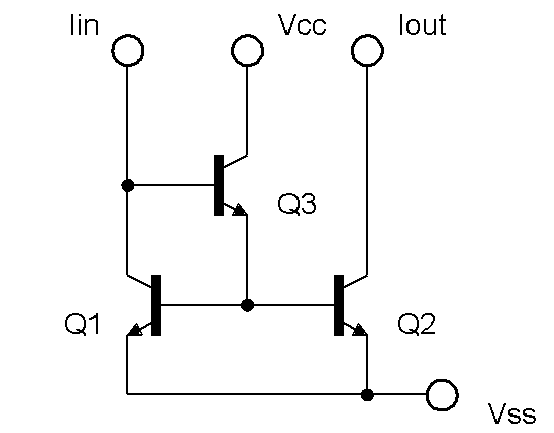
\includegraphics[scale=0.5]{pict/ZlepseneWilsonovoZrcadloNPN}
%   \end{center}
%   \caption[Wilson mirror]{Improved Wilson current mirror.}
% \end{figure}

% For inclusion of the vector-based graphics directly via \LaTeX, it is possible to use the \href{https://www.ctan.org/pkg/pgf}{\texttt{TikZ}} package.
% Examples of use can be found at the \href{http://www.texample.net/tikz/examples/}{\TeX{}ample} site.
% TikZ graphics creation is supported in QTikz and TikzEdt software.




% \chapter{Examples of Listing Computer Codes}

% \section{Package \texttt{listings}}

% Listing computer codes can be handled efficiently via the \href{https://www.ctan.org/pkg/listings}{\texttt{listings}} package.
% This package introduces a new environment \texttt{lstlisting} for typesetting computer codes, as for example:
% %
% \begin{lstlisting}[language={[LaTeX]TeX}]
% \section{Package lstlistings}
% Listing computer codes can be handled efficiently
% via the \texttt{listings} package.
% This package introduces a new environment
% \texttt{lstlisting} for typesetting computer codes.
% \end{lstlisting}
% %
% The package supports a number of programming languages.
% The code to be typeset can be input directly from files on disk.
% The package allows row numbering and extracting only selected parts of the code.
% The following paragraph is an example of the use of \texttt{listings}:
% \bigskip

% \noindent
% Abbreviations are typeset with the \texttt{acronym} environment:
% \label{lst:abbrevs}
% \lstinputlisting[language={[LaTeX]TeX}, nolol, numbers=left, firstnumber=6, firstline=6, lastline=6]{text/abbreviation.tex}
% %
% The width of the input parameter, \verb|HowMuchSpace|, determines the width of the first column.
% An example of the definition of abbreviation \acs{symfs} is in Listing~\ref{lst:symfs}.

% \shorthandoff{-}
% \lstinputlisting%
% 	[language={[LaTeX]TeX}, frame=single, caption={[Example of code listing]Example of code listing.}, label=lst:symfs, numbers=left, linerange={bsymfvz-\%\%\%\ esymfvz}, includerangemarker=false]{text/abbreviation.tex}
% \shorthandon{-}

% \noindent
% The list is finished with the end of the environment:
% \lstinputlisting[language={[LaTeX]TeX}, nolol, numbers=left, firstnumber=26, linerange=26]{text/abbreviation.tex}

% \vspace{\fill}

% %\noindent
% %{\bf Poznámka k~výpisům s~použitím volby jazyka \verb|czech| nebo \verb|slovak|:}\newline
% %Pokud Váš zdrojový kód obsahuje znak spojovníku \verb|-|, pak překlad může skončit chybou.
% %Ta je způsobená tím, že znak \verb|-| je v~českém nebo slovenském nastavení balíčku \verb|babel| tzv.\ aktivním znakem.
% %Přepněte znak \verb|-| na neaktivní příkazem \verb|\shorthandoff{-}| těsně před výpisem a hned za ním jej vraťte na aktivní příkazem \verb|\shorthandon{-}|.
% %Podobně jako to je ukázáno ve zdrojovém kódu šablony.


% \clearpage

% %\section{Listing Matlab code}
% Listing \ref{lst:priklad.vypis.kodu.Matlab} contains an example of code for Matlab,
% whereas in Listing \ref{lst:priklad.vypis.kodu.C} you find an example in the C~language.

% \lstnewenvironment{matlab}[1][]{%
% \lstset{language=Matlab,numbers=left,#1}%
% }{%
% }

% \begin{matlab}%
% 	[frame=single, float=htbp, caption={[Example of the Schur--Cohn test of stability in Matlab]Example of the Schur--Cohn test of stability in Matlab.}, label=lst:priklad.vypis.kodu.Matlab, numberstyle=\scriptsize, numbersep=7pt]
% %% Priklad testovani stability filtru

% % koeficienty polynomu ve jmenovateli
% a = [ 5, 11.2, 5.44, -0.384, -2.3552, -1.2288];
% disp( 'Polynom:'); disp(poly2str( a, 'z'))

% disp('Kontrola pomoci korenu polynomu:');
% zx = roots( a);
% if( all( abs( zx) < 1))
%     disp('System je stabilni')
% else
%     disp('System je nestabilni nebo na mezi stability');
% end

% disp(' '); disp('Kontrola pomoci Schur-Cohn:');
% ma = zeros( length(a)-1,length(a));
% ma(1,:) = a/a(1);
% for( k = 1:length(a)-2)
%     aa = ma(k,1:end-k+1);
%     bb = fliplr( aa);
%     ma(k+1,1:end-k+1) = (aa-aa(end)*bb)/(1-aa(end)^2);
% end

% if( all( abs( diag( ma.'))))
%     disp('System je stabilni')
% else
%     disp('System je nestabilni nebo na mezi stability');
% end
% \end{matlab}

% \noindent
% \begin{minipage}{\linewidth}


% %\section{Listing C code}

% \begin{lstlisting}%
% 	[frame=single, numbers=right, caption={[Example of implementation of first canonical form in~C]Example of implementation of first canonical form in~C.}, label=lst:priklad.vypis.kodu.C, basicstyle=\ttfamily\small, keywordstyle=\color{black}\bfseries\underbar]
% // first canonical form
% short fxdf2t( short coef[][5], short sample)
% {
% 	static int v1[SECTIONS] = {0,0},v2[SECTIONS] = {0,0};
% 	int x, y, accu;
% 	short k;

% 	x = sample;
% 	for( k = 0; k < SECTIONS; k++){
% 		accu = v1[k] >> 1;
% 		y = _sadd( accu, _smpy( coef[k][0], x));
% 		y = _sshl(y, 1) >> 16;

% 		accu = v2[k] >> 1;
% 		accu = _sadd( accu, _smpy( coef[k][1], x));
% 		accu = _sadd( accu, _smpy( coef[k][2], y));
% 		v1[k] = _sshl( accu, 1);

% 		accu = _smpy( coef[k][3], x);
% 		accu = _sadd( accu, _smpy( coef[k][4], y));
% 		v2[k] = _sshl( accu, 1);

% 		x = y;
% 	}
% 	return( y);
% }
% \end{lstlisting}
% \end{minipage}



% \chapter{Algorithms}

% For typesetting algorithms/pseudocode, the \texttt{algorithm2e} package can be used, offering rich options.
% Algorithms can be referenced by usual cross-references, as here: see Alg.~\ref{alg:PHADQ}.

% \RestyleAlgo{ruled}
% \begin{algorithm}%[h]
% 	\DontPrintSemicolon
% 	%
% 	\caption{B-PHADQ}
% 	\label{alg:PHADQ}
% 	%
% 	Choose parameters
% 	$\tau, \sigma, > 0, \ \rho \in [0, 1]$\\
% 	Initialize $x^{(0)}, p^{(0)}, q^{(0)}$ and $\omega_\mathbf{s}$
% 	\\
% 	\For{$i=0,1,\dots$}{
% 		$q^{(i+1)}=\textup{clip}_\lambda(q^{(i)}+\sigma DR_{\omega_\mathbf{s}}G_g x)$
% 		\;
% 		$u = p^{(i)}-\tau G^*_g R^*_{\omega_\mathbf{s}}D^*q^{(i+1)}$ ~\,\%\,auxiliary
% 		\;
% 		$p^{(i+1)} = \textup{proj}_\Gamma(u)$ ~\,\%\,consistent
% 		\;
% 		$p^{(i+1)} = \frac{1}{\tau+1}(\tau \ \textup{proj}_\Gamma(u)+u)$ ~\,\%\,inconsistent
% 		\;
% 		$x^{(i+1)} = p^{(i+1)}+\rho(p^{(i+1)}-p^{(i)})$
% 	}
% 	\Return{$p^{(i+1)}$}
% \end{algorithm}



% \chapter{Content of the electronic attachment}
% An electronic attachment is often a~part of the thesis.
% The attachment is uploaded in the BUT information system together with the thesis PDF.
% Please use an appropriate file format for the attachment.

% It is suggested to comment on every folder, to specify which of the files contains main settings,
% to specify which is the main or executable file, what was the setting of the compiler etc.
% It is also valuable to specify in which version of the software the code has been tested (e.g.\ Matlab 2018b).
% In the case that hardware has been created within the thesis, the electronic attachment must contain all documentation
% (for example Eagle files with the printed circuit board layout).

% If your attachment contains a~lot of files or folders,
% \LaTeX{} package \href{https://www.ctan.org/pkg/dirtree}{\texttt{dirtree}} can become handy,
% as in the following example.

% \bigskip

% {\small
% %
% \dirtree{%.
% .1 /\DTcomment{root of the attached archive}.
% .2 logo\DTcomment{logotypes}.
% .3 BUT\_abbreviation\_color\_PANTONE\_EN.pdf.
% .3 BUT\_color\_PANTONE\_EN.pdf.
% .3 FEEC\_abbreviation\_color\_PANTONE\_EN.pdf.
% .3 UTKO\_color\_PANTONE\_EN.pdf.
% .2 pdf\DTcomment{PDFs (generate them in the information system)}.
% .3 assignment-example.pdf.
% .3 cover-example.pdf.
% .3 titlepage-example.pdf.
% .2 pict\DTcomment{other graphic files}.
% .3 soucastky.png.
% .3 spoje.png.
% .3 ZlepseneWilsonovoZrcadloNPN.png.
% .3 ZlepseneWilsonovoZrcadloPNP.png.
% .2 text\DTcomment{\LaTeX{} source codes of the text}.
% .3 abbreviation.tex.
% .3 appendix.tex.
% .3 bibliography.tex.
% .3 conclusion.tex.
% .3 introduction.tex.
% .3 results.tex.
% .3 solution.tex.
% .2 template-thesis.tex\DTcomment{main file of the thesis}.
% .2 template-presentation.tex\DTcomment{main file of the slides for presentation}.
% .2 thesis.sty\DTcomment{package for typesetting final theses at BUT}.
% }
% }
